\documentclass{article}

\textwidth=6.5in
\textheight=8.5in
\voffset=-54pt
\oddsidemargin=0in
\evensidemargin=0in
\setlength{\parskip}{8pt}
\setlength{\parindent}{0pt}

\usepackage{amsmath, amssymb}
\usepackage{ifthen}

\usepackage[inline]{enumitem}
\setlist{topsep=0pt, parsep=8pt}

\usepackage[rgb,table]{xcolor}\convertcolorsUfalse
\usepackage{graphicx}

% change hyperref options
\PassOptionsToPackage{hyphens}{url}
\usepackage[bookmarks,colorlinks,linkcolor=black,citecolor=blue,pdfstartview=FitH,urlcolor=blue]{hyperref}
\hypersetup{pdfpagemode=UseNone}
\usepackage{bookmark}

\usepackage{graphicx}
\usepackage{multicol}
\usepackage{framed}
\usepackage{array}

\usepackage{icomma}

\usepackage{soul}
\usepackage[normalem]{ulem}

\usepackage{pgfplots}
\pgfplotsset{compat=1.18}  
\pgfplotscreateplotcyclelist{mycolor}{black, blue, red, green!70!black, magenta, purple, cyan, orange }  
\pgfplotsset{
  disabledatascaling,
  cycle list=tikzcolor, 
  axis lines=middle,
  every axis plot/.style={no marks, thick},
  every axis/.style={
    enlarge x limits=false,
    enlarge y limits=auto,
    xlabel style={at={(current axis.right of origin)},anchor=west},
    ylabel style={at={(current axis.above origin)},anchor=south},
    % extra x and y ticks for asymptotes
    extra x tick style={grid=major, grid style={dashed,black}},
    extra y tick style={grid=major, grid style={dashed,black}},
    /pgf/number format/1000 sep={},
  },    
  tick label style = {font=\footnotesize, fill=\currentbgcolor, inner sep=0pt},    
  xticklabel shift=1pt,    
  scaled ticks=false,
  scaled y ticks=false,
  unbounded coords=jump,
  samples=101,
  minor tick length=0,
  scatter/classes={
    open={mark=*,draw=black,fill=white, mark size=2, thin},
    closed={mark=*,draw=black,fill=black, mark size=2, thin}
  },
  width=3in,
}
\pgfplotsset{open/.style={only marks, mark=*, fill=white, thin, mark size=2}}
\pgfplotsset{closed/.style={only marks, mark=*, draw=black, fill=black,
    thin, mark size=2}}
\pgfplotsset{labeled/.style={nodes near coords, only marks, mark=*, draw=black, fill=black, thin, mark size=2, point meta=explicit symbolic}}

\pgfplotsset{gridgraph/.style={clip=false, axis line style={shorten
      >=-8pt}, xlabel style={xshift=8pt}, ylabel style={yshift=8pt},
    enlargelimits=false, grid=major, tick style={black}}} 

\newcommand{\axes}[1][]{
  \begin{tikzpicture}
    \begin{axis}[xtick=\empty, ytick=\empty, ymin=-2, ymax=2,
      xmin=-4.25, xmax=4.25, #1]
    \end{axis}
  \end{tikzpicture}
}

\usepackage{tikz}
\usetikzlibrary{
  matrix,%
  % enables the snake paths
  decorations.pathmorphing,%
  % enables bigger arrows
  decorations.markings,%
  decorations.pathreplacing,%
  decorations.text,%
  calc,%
  patterns,%
  shapes.geometric,%
  arrows,
  decorations.shapes,
  positioning,
  plotmarks,
  intersections
}
\tikzset{>=latex} % sets default arrow type in tikz
\tikzset{font=\normalsize}
\tikzset{mark size=1.5pt, mark options=thin}
\tikzset{pin distance=4pt,
  every pin edge/.style={<-, thin, shorten <= -2pt}}

\interfootnotelinepenalty=10000
\renewcommand{\thefootnote}{(\arabic{footnote})}

\usepackage{multirow, bigdelim}

% change to \usepackage[sols]{handout} to see solutions
\usepackage[]{handout}

\newcommand\iscurrentenumi[1]{%
  \ifthenelse{\equal{#1}{\theenumi}}{}{#1}}
\setenumerate[1]{ref=\#\arabic*}
\setenumerate[2]{ref=\protect\iscurrentenumi{\theenumi}(\alph*)}
\newcommand\enumiiprefix[2]{%
  \ifthenelse{{\equal{#1}{\theenumi}}\AND{\equal{#2}{(\alph{enumii})}}}{}{}%
  \ifthenelse{{\equal{#1}{\theenumi}}\AND{\NOT{\equal{#2}{(\alph{enumii})}}}}{#2}{}%
  \ifthenelse{\equal{#1}{\theenumi}}{}{#1#2}%
}
\setenumerate[3]{ref=\protect\enumiiprefix{\theenumi}{(\alph{enumii})}\roman*}

\usepackage{tabto}

\newlength{\tipmargin}
\makeatletter

\renewenvironment{framed}{
  \setlength{\tipmargin}{\textwidth-\linewidth}
  \advance\@totalleftmargin-\tipmargin
  \def\FrameCommand{\hspace{\tipmargin}\fbox}%
  \advance\linewidth\tipmargin
  \MakeFramed {\advance\hsize-\width \FrameRestore}%
}
{\endMakeFramed}

\makeatother

\definecolor{purple}{rgb}{0.5,0,1.0}

\newlength{\dwidth}
\usepackage{fourier-orns}

\usepackage{fancyhdr}
\lhead{\textcolor{white}{This content is protected and may not be shared, uploaded, or distributed.}}
\rhead{}
\rfoot{\vspace*{\fill}\footnotesize\textcopyright{} \emph{Harvard Math Ma}}
\renewcommand{\headrulewidth}{0pt}
\pagestyle{fancy}
\begin{document}

\htitle{29. Introduction to Logarithms}

\begin{problemonly}
  \begin{framed}

You should be able to:
    \begin{itemize}[topsep=0pt,partopsep=0pt,parsep=8pt,itemsep=0pt]
    \item State and apply the definition of a logarithm, and explain how logarithms are related to exponentials.

    \item Explain how to simplify $\log_b \left( b^{\bigstar} \right)$ and $b^{\log_b \heartsuit}$.

    \item Sketch $y = \log_b x$ and explain how the graph and its important features (domain, range, asymptotes, intercepts, etc.)\ relate to the graph of $y = b^x$.

    \item Differentiate $b^x$ for any constant $b > 0$.

    \end{itemize}
  \end{framed}
\end{problemonly}

\begin{enumerate}
\item  \label{tech-exponential}

  \note{We'll do this fairly quickly. I want students to see that we
    want to solve $1.03^t = 2$, and from the graph of $1.03^t$, there
    should definitely be such a value. I'll let them know it's about
    23, but we'd like a name for the exact quantity, and I'll
    introduce the notation $\log_{1.03} (2)$.}

  % This data comes from http://blogs.zdnet.com/BTL/?p=6195 and
  % http://www.nytimes.com/2007/10/25/technology/25facebook.html 

  \begin{problem}[\vfill]
    When a new technology (like iPhones, Facebook, Twitter, etc.)\ starts to become popular, it often experiences exponential growth. In 2007, Facebook reported that the number of Facebook members was growing by about 3\% per week. On October 25 of that year, Facebook reached 50 million members; if the growth trend continued, when did the number of members reach 100 million?
  \end{problem}

  \begin{solution}
    Let's do this in terms of weeks; $t$ weeks after October 25, 2007, 
    Facebook ought to have $50 \cdot 1.03^t$ million members.  We are
    interested in the value of $t$ making this equal to 100 million; that
    is, we want $50 \cdot 1.03^t = 100$, or $1.03^t = 2$.

    We don't know how to find this exactly, but in words, we are looking
    for the power $t$ to which $1.03$ must be raised in order to get $2$.
    We write this as $\boxed{\log_{1.03} 2}$.
  \end{solution}

\item  \label{log-intro}

  \note{I will have students try this.}

  \begin{enumerate}
  \item We read $\log_{7} (40)$ as ``\fitb{2in}{log base 7 of 40}.''

    This number is the power to which \fitb{0.5in}{7} must be raised in order to get \fitb{0.5in}{40}.

    Find upper and lower bounds for this number: $\fitb{0.5in}{1} < \log_7 (40) < \fitb{0.5in}{2}$.

    \pspace{0.5in}

  \item Evaluate the following.

    $\log_7 (49) = \fitb{1in}{2}$ \qquad $\displaystyle \log_7 \left( \frac{1}{\sqrt{7}} \right) = \fitb{1in}{-1/2}$ \qquad $\log_7 (1) = \fitb{1in}{0}$

    \pspace{0.5in}

    Make up two more examples, one where the log is positive and one where it's negative:

    $\log_7 \left( \fitb{0.5in}{7} \right)= \fitb{0.5in}{1}$ \qquad $\displaystyle \log_7 \left( \cfitb{0.5in}{\frac{1}{7}} \right) = \fitb{0.5in}{-1}$

    \pspace{0.5in}

    \pspace{\newpage}

  \item If $\log_7 (v) = w$, then $\fitb{0.35in}{w}$ is the power to which $\fitb{0.35in}{7}$ must be raised in order to get $\fitb{0.35in}{v}$. This can be rewritten as an exponential equation 
  \probonly{$\vphantom{\boxed{int_1^2}}$}$\fitb{1.25in}{7^w=v}$.

  \item \label{log-intro-relation-to-exp}
    \begin{problem}[\stretch{0.5}]
      If $f(x) = \log_7 (x)$, find $f^{-1}(x)$. 
    \end{problem}

    \begin{solution}
      To find $y=f^{-1}(x)$, we need to solve $f(y)=x$ for $y$.
      \begin{align*}
        \log_7 y &= x \\
        7^x &= y
      \end{align*}
      Therefore $f^{-1}(x) = 7^x$.
    \end{solution}

  \item
    \begin{problem}[\vfill]
      Use your answer to \ref{log-intro-relation-to-exp} to graph $y = \log_7 (x)$, and label at least 3 points on your graph.
    \end{problem}

    \begin{problem}
      \NumTabs{2}
      What's the domain of $\log_7 (x)$? 
      \tab What's the range of $\log_7 (x)$?

      Where are its intercepts? \hspace{1in}
      \tab Does it have any asymptotes?
    \end{problem}

    \begin{solution}
      The graph of of $y=\log_7 x$ is the graph of $y=7^x$
      reflected over the line $y=x$. We found several
      points on the graph in part (b),
      e.g. $(\frac{1}{7},0)$, $(1, 0)$, and $(7, 0)$. 

      \begin{center}
        \begin{tikzpicture}
          \begin{axis}[ytick={-1,1}, xtick={1,7}]
            \addplot[domain=0:10,samples=300] {ln(x)/ln(7)};
            \addplot[closed] coordinates {(1/7,-1) (1,0) (7,1)};
            \node[right] at (1/7,-1) {$(\frac{1}{7},-1)$};
          \end{axis}
        \end{tikzpicture}
      \end{center}
      The domain of the function is $(0, \infty)$ and the range
      is $(-\infty, \infty)$. The $x$-intercept is $(1,0)$, and
      there are no $y$-intercepts. There is a vertical asymptote,
      $x=0$.
    \end{solution}

  \item

    \note{Here are some basic consequences of $\log_7 x$ and $7^x$ being inverse functions. The first one is obvious from the definition of $\log_7$, but the second one can feel more mysterious to students.}

    \begin{problem}[0.5in]
      What's $\log_7 \left( 7^\bigstar \right)$? 
      $\fitb{0.5in}{\bigstar}$ \tab What's
      $7^{\log_7 (\heartsuit)}$? $\fitb{0.5in}{\heartsuit}$
    \end{problem}

  \end{enumerate}

\end{enumerate}
\begin{framed}
  \emph{Notation for a special base.}  We call the base $e$ logarithm
  the ``natural logarithm'' and write $\ln(x)$ as shorthand for $\log_e (x)$.
  So, $\ln (x)$ is the power to which \fitb{0.25in}{$e$} must be raised
  in order to get \fitb{0.25in}{$x$}.
\end{framed}

\begin{enumerate}[resume]
\item  Make up a few examples, including one where the natural log is positive and one where it's negative:

  $\ln \left( \fitb{0.5in}{\frac{1}{e}} \right) = \fitb{0.5in}{-1}$
  \qquad $\ln \left( \fitb{0.5in}{1} \right) = \fitb{0.5in}{0}$ \qquad $\ln \left( \fitb{0.5in}{e} \right) = \fitb{0.5in}{1}$

  \pspace{0.25in}

  \pspace{\newpage}

\item 
  \begin{problem}[\stretch{1.25}]
    Usually, when we have a function $f$, it is \uline{not} considered acceptable to write $f x$ instead of $f(x)$. However, with logarithmic functions, it is! So, $\log_7 40$ is a common notation for $\log_7(40)$, and $\ln(5)$ is commonly written as $\ln 5$.

    However, it \textbf{isn't} okay to write an expression like $\log_5 x^2$ because it's ambiguous. What are 2 ways a reader might interpret $\log_5 x^2$? What would each interpretation equal if $x = 5$?
  \end{problem}

  \begin{solution}
    $\log_5 x^2$ could be interpreted as $\log_5 (x^2)$ or as
    $(\log_5 x)^2$. If $x=5$, then $\log_5 (5^2)=\log_5 25 = 2$,
    but $(\log_5 5)^2 = (1)^2 = 1.$
  \end{solution}

\end{enumerate}
\begin{framed}
  \danger In different sources, you may encounter the notation $\log(x)$, where no base is written. This doesn't have a single set meaning! In the Gottlieb textbook, this means $\log_{10} (x)$. But in other sources, it might mean $\log_2 (x)$ or $\log_e (x)$. We'll avoid this notation in Math Ma. 
\end{framed}

\begin{enumerate}[resume]
\item  

  \note{This is to introduce students to the idea that every exponential function can be written as $f(t) = C e^{kt}$.}

  In \ref{tech-exponential}, the number of millions of Facebook users $t$ weeks after October 25 was $50 \left( 1.03^t \right)$.

  \begin{enumerate}

  \item
    \begin{problem}[\vfill]
      Can you write $1.03$ as $e^k$ for some $k$?  If so, what's $k$? 
    \end{problem}

    \begin{solution}
      We are essentially solving the equation $e^k = 1.03$.
      We can express the solution as $k=\ln(1.03)$, the exponent
      to which $e$ must be raised to get $1.03$. 
    \end{solution}

  \item
    \begin{problem}[0.35in]
      Rewrite $50 \left( 1.03^t \right)$ in the form $C e^{kt}$.
    \end{problem}

    \begin{solution}
      Since $1.03 = e^{\ln(1.03)}$,
      \[50(1.03)^t  = 50(e^{\ln(1.03)})^t = 50e^{\ln(1.03)t},\]
      with $C=50$ and $k=\ln(1.03)$.
    \end{solution}

  \end{enumerate}

\end{enumerate}
\begin{framed} \label{summary:exp-2-forms}
  Every exponential function can be written as $f(x) = \fitb{0.5in}{C \cdot b^x}$ or as $f(x) = \fitb{0.5in}{C e^{kx}}$.  
\end{framed}

\begin{enumerate}[resume]
\item  We can use the boxed fact to find the derivative of $7^x$!

  \begin{enumerate}
  \item
    \begin{problem}
      So far, what do we know about $\frac{d}{dx} 7^x$?   
      \vfill
    \end{problem}

    \begin{solution}
      We know that $\frac{d}{dx} 7^x$ is proportional to
      $7^x$, so $\frac{d}{dx} 7^x = b \cdot 7^x$. The proportionality constant $b$ is the slope
      of the line tangent to $y=7^x$ at $x=0$. 
    \end{solution}

  \item
    \begin{problem}
      What's $\frac{d}{dx} e^{kx}$?
      \vfill
    \end{problem}

    \begin{solution}
      $\frac{d}{dx} e^{kx} = ke^{kx}$.
    \end{solution}

  \item    
    \begin{problem}[\nstretch{1.25}]
      Rewrite $7^x$ in the form $C e^{kx}$, and use this to find $\frac{d}{dx} 7^{x} $.
      \vfill 
    \end{problem}

    \begin{solution}
      Similar to \#5, we can rewrite $7^x$ as $e^{\ln(7)x}$.
      This means that
      \begin{align*}
        \frac{d}{dx} 7^x &= \frac{d}{dx} e^{\ln(7)x} \\
        &= \ln(7) \cdot e^{\ln(7)x}\\
        &= \ln(7) \cdot 7^x
      \end{align*}
    \end{solution}

  \end{enumerate}

\end{enumerate}
\begin{framed}
  If $b > 0$, then
  $\frac{d}{dx} b^x = 
  \fitb[\vphantom{\dfrac{1}{1}}]{1.5in}{\ln(b) \cdot b^x}$
\end{framed}

\begin{enumerate}[resume]
\item  \label{simplify-exp-of-log-expressions-1}

  Simplify the following expressions. (One is already simplified!)

  \begin{enumerate}

  \item

    \note{This one is very concrete, but it's a chance to point out that this agrees with the fact $7^{\log_7 \heartsuit} = \heartsuit$ that we figured out earlier.}

    \begin{problem}[\vfill]
      $7^{\log_7 49}$
    \end{problem}

    \begin{solution}
      $7^{\log_7 49}=49$. We know this because $\log_7 49 = 2$, 
      but also because $7^{\log_7 \heartsuit} = \heartsuit$.
    \end{solution}

  \item
    \begin{problem}[\vfill]
      $e^{\ln 2}$
    \end{problem}

    \begin{solution}
      $e^{\ln 2}=2$. We know this because $e^{\ln \heartsuit} =
      \heartsuit$
    \end{solution}

  \item

    \note{I hope to get to at least this part because it's tempting for students to say this is $6 + 7 = 13$. If that happens, I will try to have students realize that $\log_5 6$ and $\log_5 7$ are both bigger than 1, so $\log_5 6 + \log_5 7$ should be at least 2, which means this expression should be at least $5^2 = 25$.}

    \begin{problem}[\vfill]
      $5^{\log_5 6 + \log_5 7}$
    \end{problem}

    \begin{solution}
      We would like to use our rule that 
      $5^{\log_5 \heartsuit} = \heartsuit$, but notice that
      the exponent of $5^{\log_5 6 + \log_5 7}$ is \textbf{not} in
      the form $\log_5 \heartsuit$, so we can't apply the rule yet.
      We need to first use exponent rules to rewrite
      $5^{\log_5 6 + \log_5 7}$:
      \begin{align*}
        5^{\log_5 6 + \log_5 7} &= 5^{\log_5 6} \cdot 5^{\log_5 7} \\
        &= 6 \cdot 7 \\
        &= 42
      \end{align*}
    \end{solution}

  \item

    \note{Similarly, it can be tempting for students to say this is $3 \cdot 10 = 30$. But since $\log_6 10 > 1$, this should be at least $6^3$.}

    \begin{problem}[\vfill]
      $6^{3 \log_6 10}$
    \end{problem}

    \begin{solution}
      Again, we would like to apply the rule that 
      $6^{\log_6 \heartsuit} = \heartsuit$, but the exponent of
      $6^{3 \log_6 10}$ is \textbf{not} in the form $\log_6 \heartsuit$.
      We need to first use exponent rules to rewrite it $6^{3 \log_6 10}$:
      \begin{align*}
        6^{3\log_6 10} &= (6^{\log_6 10})^3 \\
        &= (10)^3 \\
        &= 1000
      \end{align*}
    \end{solution}

  \item
    \begin{problem}[\vfill]
      $3^{\log_7 3}$
    \end{problem}

    \begin{solution}
      There isn't anything we can do to simplify this.
    \end{solution}

  \item
    \begin{problem}[\vfill\newpage]
      $e^{{-\ln 3}}$
    \end{problem}

    \begin{solution}
      \begin{align*}
          e^{-\ln 3} &= (e^{\ln 3})^{-1} \\
          &= (3)^{-1} \\
          &= \tfrac{1}{3}
      \end{align*}
    \end{solution}

  \end{enumerate}

\item 

  As we saw on page \pageref{summary:exp-2-forms}, every exponential function $f$ can be written as $f(x) = C \cdot b^x$ and as $f(x) = C e^{kx}$. This is useful because we know how to find the derivative of both $C \cdot b^x$ and $C e^{kx}$. Rewrite each function below in both forms, and then find its derivative.

  \begin{enumerate}
  \item
    \begin{problem}[\vfill]
      $f(x) = 5^{2x - 1}$
    \end{problem}

    \begin{solution}
      First, we can rewrite $f(x)$ into the form $C \cdot b^x$.
      \begin{align*}
        5^{2x-1} &= 5^{2x} \cdot 5^{-1} \\
        &= \tfrac{1}{5} (5^2)^x
      \end{align*}
      Using our rule that $\frac{d}{dx} b^x = \ln(b) \cdot b^x$,
      \begin{align*}
        \tfrac{d}{dx} 5^{2x-1} &= 
        \tfrac{d}{dx}\! \left(\tfrac{1}{5}\cdot (5^2)^x\right) \\
        &= \tfrac{1}{5} \ln(5^2)(5^2)^x
      \end{align*}

      We can also find the derivative by rewriting
      $5^{2x-1}$ into the form $Ce^{kx}$.
      \begin{align*}
           \tfrac{d}{dx} 5^{2x-1} &= 
           \tfrac{d}{dx}\!\left(\tfrac{1}{5} \cdot (5^2)^x\right) \\
           &=\tfrac{d}{dx}\!\left( \tfrac{1}{5} e^{\ln(5^2)x}\right) \\
           &= \tfrac{1}{5}\ln(5^2)e^{\ln(5^2)x}
      \end{align*}
      The derivatives that we found look a bit different, but
      you can check that they are equivalent using exponent rules.
    \end{solution}

  \item
    \begin{problem}[\vfill]
      $g(x) = 7 e^{3x + 2}$
    \end{problem}

    \begin{solution}
      First, let's find $g'(x)$ by rewriting $g(x)$ into the form 
      $Ce^{kx}$.
      \begin{align*}
          \tfrac{d}{dx}\! \left(7e^{3x+2}\right) &= 
          \tfrac{d}{dx}\! \left(7e^2e^{3x}\right) \\
          &= 7e^2(3e^{3x})
      \end{align*}
      Now let's find $g'(x)$ by rewriting $g(x)$ into the form
      $C\cdot b^x$.
      \begin{align*}
        \tfrac{d}{dx}\! \left(7e^{3x+2}\right) &= 
          \tfrac{d}{dx}\! \left(7e^2e^{3x}\right) \\
          &= \tfrac{d}{dx}\! \left(7e^2(e^3)^x\right) \\
          &= 7e^2\left(\ln(e^3)\cdot (e^3)^x\right)
      \end{align*}
      The derivatives that we found look a bit different, but
      you can check that they are equivalent using exponent rules
      and properties of logs.
    \end{solution}

  \end{enumerate}

\item 
  \begin{enumerate}
  \item
    \begin{problem}[\stretch{2}]
      Sketch the graph of $f(x) = 4 - \log_{10} x$.  What are the intercepts
      and asymptotes of $f$?
    \end{problem}

    \begin{solution}
      The graph of $y=f(x)$ will be the graph of $y=\log_{10} x$
      reflected over the $x$-axis and shifted up by 4 units. So first,
      let's consider the graph of $y=\log_{10} x$. Some of the points
      it passes through are $(0.1, -1)$, $(1, 0)$, and $(10, 1)$.
      It has a vertical asymptote at $x=0$.
      \begin{center}
        \begin{tikzpicture}
          \begin{axis}[xtick={1}, ytick=\empty]
            \addplot[domain=0:15, samples=400] {ln(x)/ln(10)};
          \end{axis}
        \end{tikzpicture}
      \end{center}

     When we reflect over the $x$-axis and shift up by $4$ units,
     the vertical asymptote will remain at $x=0$. We can find
     the $x$-intercept by solving the equation $4-\log_{10} x = 0$.
     \begin{align*}
      4-\log_{10} x &= 0 \\
      4 &= \log_{10} x \\
      x &= 10^4
     \end{align*}
      \begin{center}
        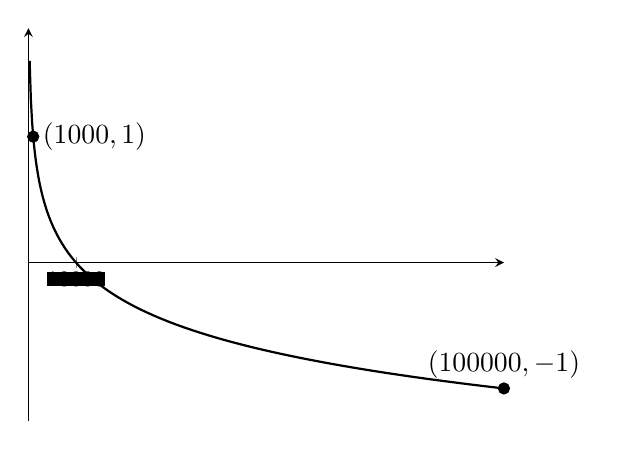
\begin{tikzpicture}
          \begin{axis}[xmin=0, xmax=1e5, xtick={1e4}, ytick=\empty,
          disabledatascaling=false, clip=false]
            \addplot[domain=0:1e5, samples=400] {4-ln(x)/ln(10)};
            \addplot[closed] coordinates {(1e3, 1) (1e5,-1)};
            \node[right] at (1e3, 1) {$(1000, 1)$};
            \node[above] at (1e5,-1) {$(100000, -1)$};
          \end{axis}
        \end{tikzpicture}
      \end{center}
    \end{solution}

  \item
    \begin{problem}[0.25in]
      Label at least three points on the graph.
    \end{problem}

    \begin{solution}
      Three points on the graph are $(1000, 1)$, $(10000,0)$ and
      $(100000,-1)$.
    \end{solution}

  \item
    \begin{problem}[\vfill]
      Is $f$ invertible? If so, find the domain and range of $f^{-1}$, as well as a formula for $f^{-1}(x)$. 
    \end{problem}

    \begin{solution}
      Since the graph passes the horizontal line test, $f$ is invertible.
      The domain of $f^{-1}$ is the same as the range of $f$, 
      $(-\infty, \infty)$. The range of $f^{-1}$ is the same as the 
      domain of $f$, $(0, \infty)$. To find a formula for $f^{-1}(x)$,
      we solve $x=f(y)$ for $y$.
      \begin{align*}
        4-\log_{10} y &= x \\
        -\log_{10} y &= x-4 \\
        \log_{10} y &= -x+4 \\
        y &= 10^{-x+4}
      \end{align*}
      Therefore $f^{-1}(x) = 10^{-x+4}$.
    \end{solution}
  \end{enumerate}

\end{enumerate}
\end{document}
